\subsection{\large{\textit{aP}4-Li (Inverse)}}\vspace{-0.1in}
Inverse Lithium


\begin{figure}[H]
\begin{minipage}{0.34\textwidth}\centering
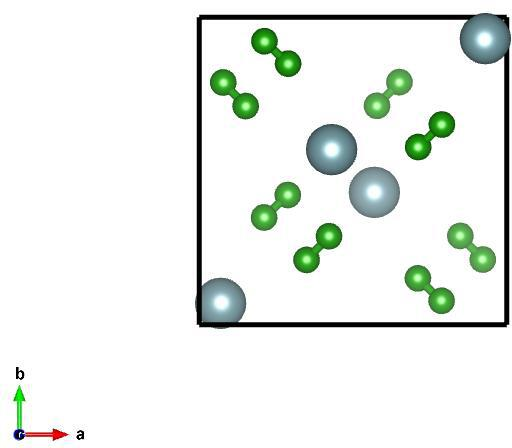
\includegraphics[width=0.9\linewidth,height=2in,keepaspectratio]{/Users/rosecers/work_folders/structures_for_photonics/reference/ref_inp/workspace/143d46cabf887052cdaf0814bfb928c6/final_images/analog_trim.jpg}\\
\small{Image of \textit{aP}4-Li, generated by Vesta}
\end{minipage}\hfill
\begin{minipage}{0.65\textwidth}\raggedright
{\setlength{\mathindent}{0cm}
\begin{equation*}
\begin{split}&\boldsymbol{a_1} = \ \hat{x} + 0.0001\ \hat{y} - 0.0004\ \hat{z}\\[-8pt]
&\boldsymbol{a_2} = 1.0009\ \hat{y}\\[-8pt]
&\boldsymbol{a_3} = 1.0003\ \hat{z}
\end{split}
\end{equation*}}

\textbf{Space Group:}	1\hspace{0.5in}\textbf{Point Group:}	$1$\\
\textbf{Found in Simulation}\\
\textbf{Structure DOI: }\url{10.1021/nn204012y}

\textbf{Photonics DOI: }\url{10.1063/1.1635664}
\end{minipage}\hfill
\end{figure}
\vspace{-0.25in}


\begin{figure}[H]
\begin{minipage}{0.9\textwidth}\centering
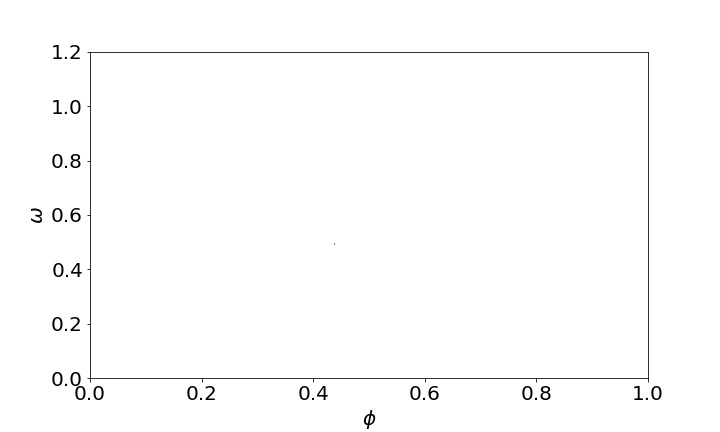
\includegraphics[width=0.9\linewidth,height=2.5in,keepaspectratio]{/Users/rosecers/work_folders/structures_for_photonics/reference/ref_inp/workspace/143d46cabf887052cdaf0814bfb928c6/final_images/gap_atlas.jpg}
\\
\end{minipage}\hfill\caption{Gap Atlas across filling fraction $\phi$ and frequency $\omega$}
\end{figure}


\begin{figure}[H]
\begin{minipage}{0.5\textwidth}\centering
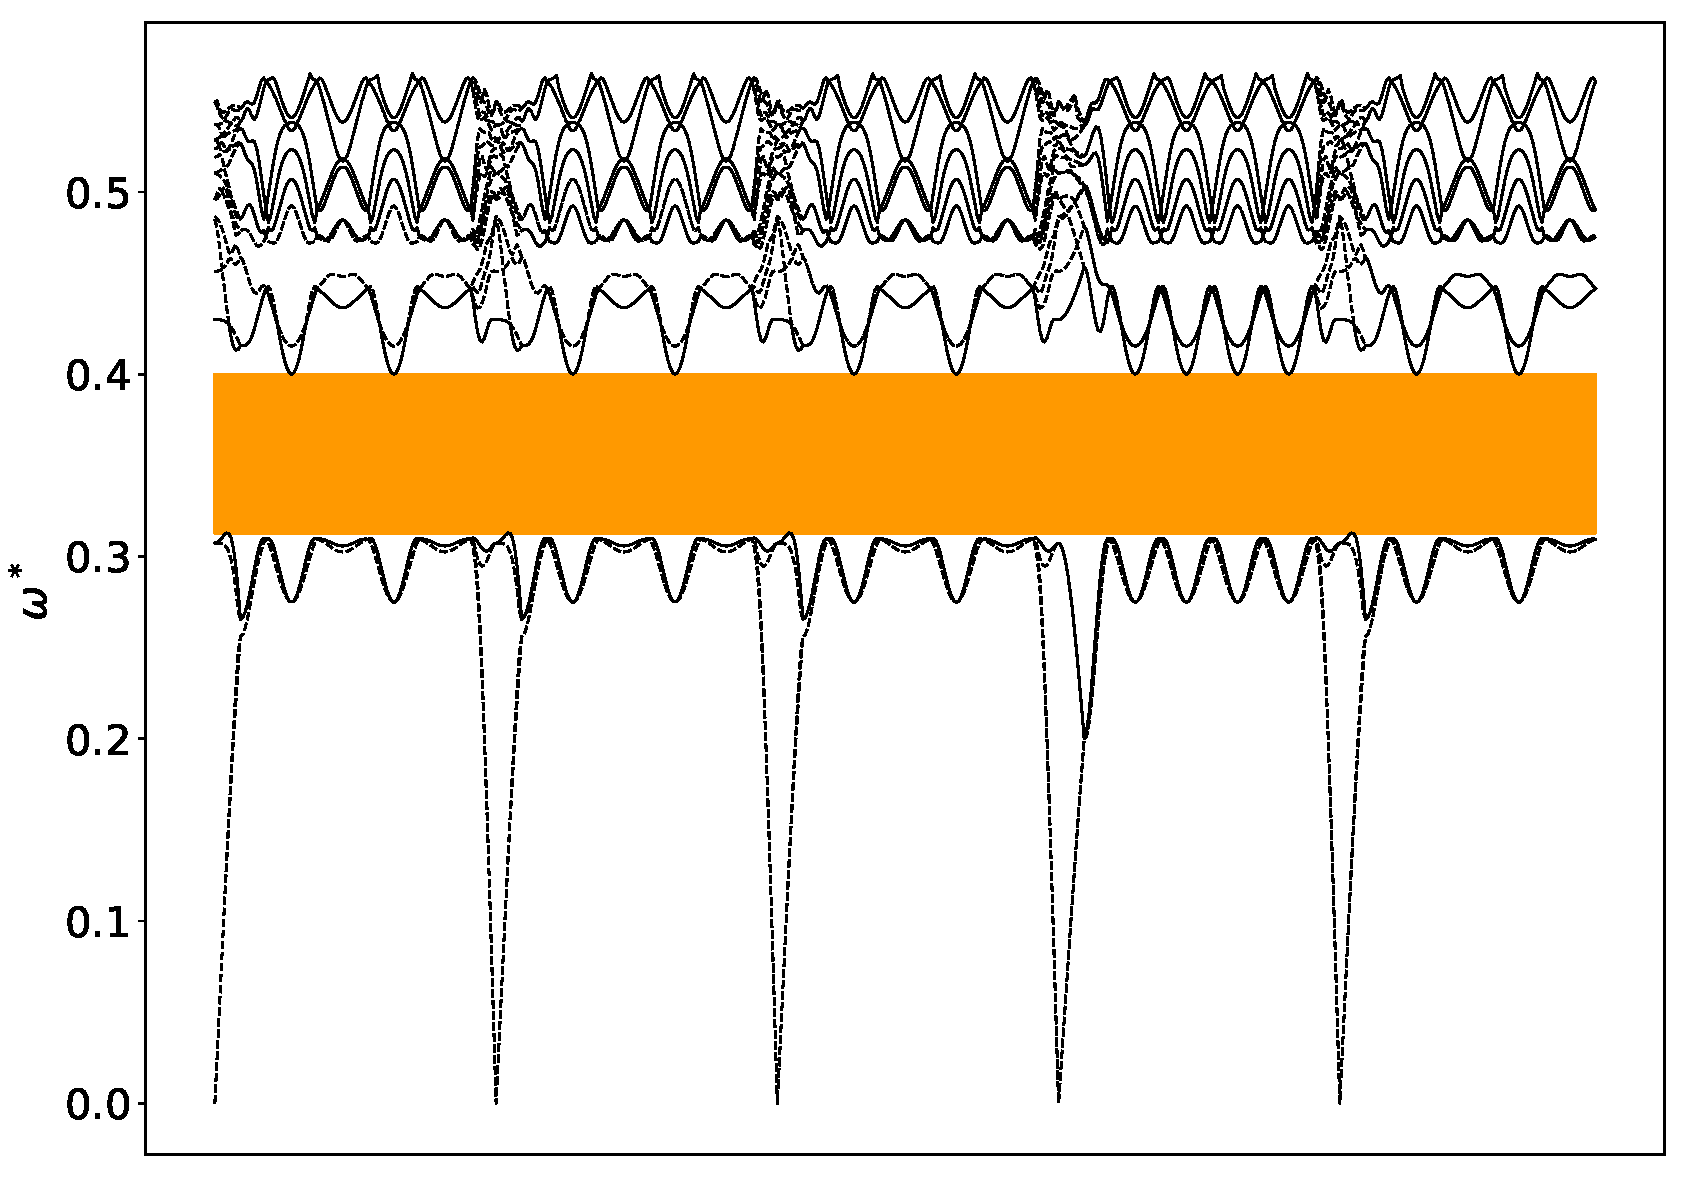
\includegraphics[width=0.9\linewidth,height=1.5in,keepaspectratio]{/Users/rosecers/work_folders/structures_for_photonics/reference/ref_inp/workspace/143d46cabf887052cdaf0814bfb928c6/./final_images/band_diagram_b=4.pdf}
\\Band Structure across 1st BZ
\end{minipage}\hfill
\begin{minipage}{0.25\textwidth}\centering
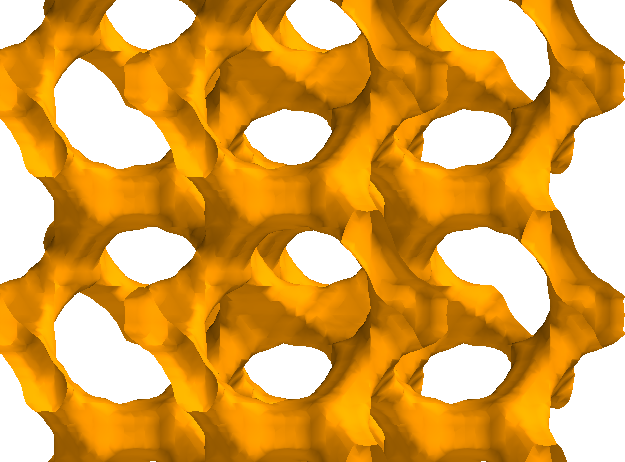
\includegraphics[width=0.9\linewidth,height=1.5in,keepaspectratio]{/Users/rosecers/work_folders/structures_for_photonics/reference/ref_inp/workspace/143d46cabf887052cdaf0814bfb928c6/final_images/aP4-Li_r@gap_4-5.png}
\\View along $a_1$ 
\end{minipage}\hfill
\begin{minipage}{0.23\textwidth}\centering
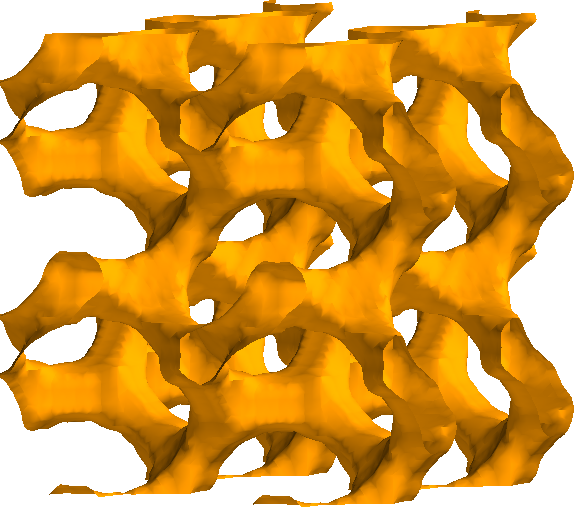
\includegraphics[width=0.9\linewidth,height=1.5in,keepaspectratio]{/Users/rosecers/work_folders/structures_for_photonics/reference/ref_inp/workspace/143d46cabf887052cdaf0814bfb928c6/final_images/aP4-Li_r@gap_4-5_1.png}
\\View rotated 140$^{\circ}$ about $l_3$  and elevated 0${\circ}$
\end{minipage}\hfill\caption{Band Structure and Isosurface of \textit{aP}4-Li (Inverse) at radius = 0.4, filling fraction = 0.164, where the largest gap between bands 4 and 5 occurs with gap size 27.07\%.}

\end{figure}
\vspace{-0.25in}

